\documentclass[12pt,a4paper,twoside]{article}
\usepackage{labor}
\begin{document}

%fill for cover and header creation
\newcommand\laboratorynumber{2}
\title{Dünne Linsen}
\newcommand\supervisor{Ditlbacher, Harald}
\newcommand\groupnumber{42}

\newcommand\participantonelastname{Eisner}
\newcommand\participantonefirstname{Nico}
\newcommand\participantoneid{12214121}
\newcommand\participanttwolastname{Waldl}
\newcommand\participanttwofirstname{Philip}
\newcommand\participanttwoid{12214120}
\author{\participantonelastname \ \& \participanttwolastname}

\newcommand\degreeid{UB 033 678}
\newcommand\semester{23WS}
\date{17.11.2023}

%select correct course title
%\newcommand\coursetitle{Einführung in die \\ physikalischen Messmethoden}
%\newcommand\coursetitle{Laborübungen 1: \\ Mechanik und Wärme}
\newcommand\coursetitle{Laborübungen 2: \\ Elektrizität, Magnetismus, Optik}
%\newcommand\coursetitle{Fortgeschrittenen Praktikum 1: \\ Technische Physik}
%\newcommand\coursetitle{Fortgeschrittenen Praktikum 2: \\ Allgemeine Physik}

%\begin{titlepage}
   \begin{center}
       \begin{figure}[H]
            \begin{minipage}[h]{30mm}
                \centerline{
\includegraphics[height=15mm]{cover_nudes/tugraz.png}}
            \end{minipage}
            \hfill
            \begin{minipage}[h]{30mm}
                \centerline{
\includegraphics[height=15mm]{cover_nudes/nawi_graz.png}}
            \end{minipage}
            \hfill
            \begin{minipage}[h]{30mm}
                \centerline{
\includegraphics[height=15mm]{cover_nudes/uni-graz.png}}
            \end{minipage}
        \end{figure}
        
        \large{\emph{Institut für Experimentalphysik der Technischen Universität Graz \\
        \& Institut für Physik der Universität Graz}} \\
        \vspace{5mm}
        
        {\Huge \textbf{\coursetitle}}
        \vspace{5mm}
        
        {\huge \laboratorynumber: \thetitle}
    \end{center}
    
    \vfill
    
    \begin{table}[H]
        \LARGE
        \centering
        \begin{tabular}{r l}
            Betreuer:       & \supervisor \\
            Gruppennummer:  & \groupnumber \\
            \\
            Name:           & \participantonelastname, \participantonefirstname \\
            Matrikelnummer: & \participantoneid \\
            Name:           & \participanttwolastname, \participanttwofirstname \\
            Matrikelnummer: & \participanttwoid \\
            \\
            Kennzahl:       & \degreeid \\
            Datum:          & \semester \ | \thedate
        \end{tabular}
    \end{table}
    \vspace{4cm}
\end{titlepage}
\clearpage
\setcounter{page}{1}

%\maketitle %short title alternative

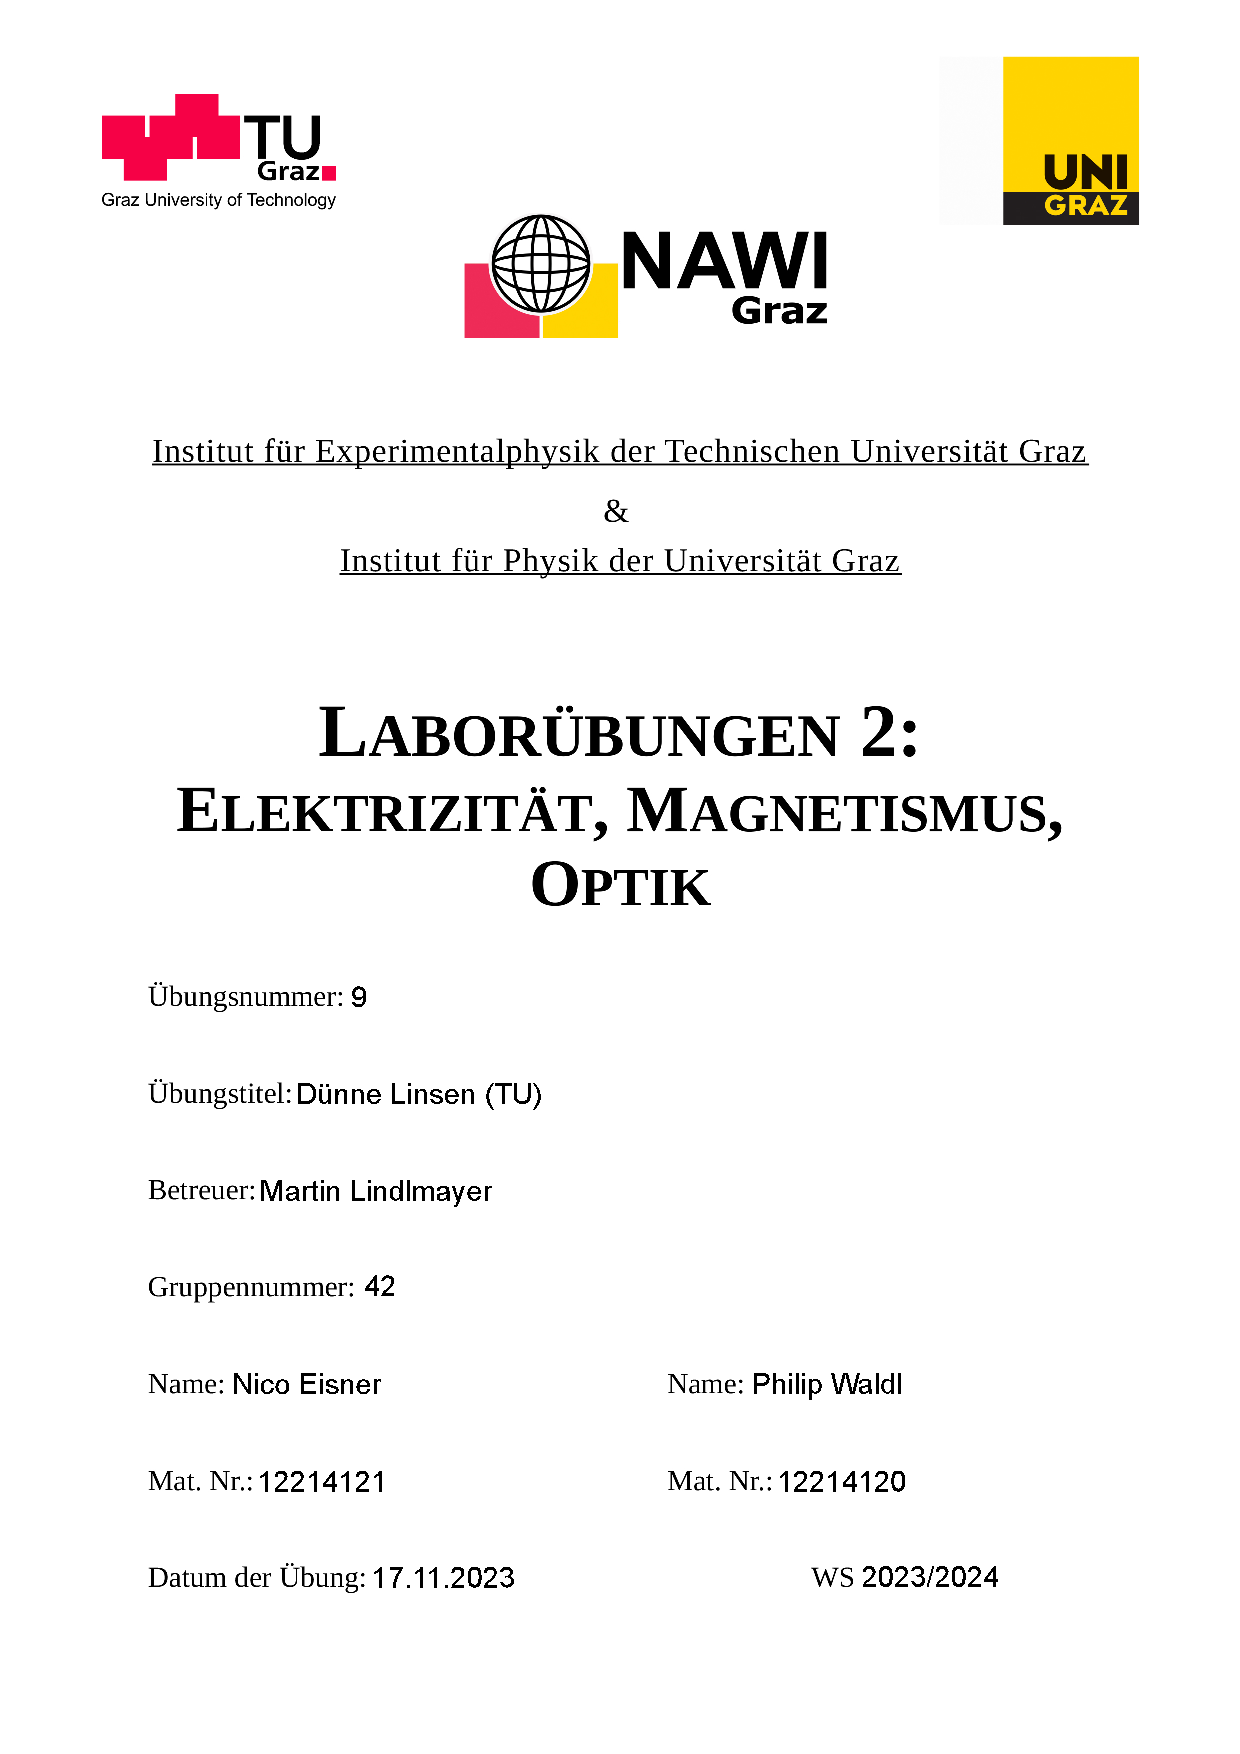
\includepdf[pages={1}]{../Deckblätter/Deckblatt_Dünne_Linsen.pdf}

\tableofcontents
\newpage

\section{Aufgabenstellung} %jo beschreibn wos gmocht host ------------------------------
Im Experiment Dünne Linsen gilt es Brennweite einer Sammellinse über zwei verschiedene Metoden zu bestimmen. 
Die Erste Methode ist jene nach der Laplace'sche Methode, die zweite nach dem Bessel'schen Verfahren. 
Desweiteren ist die Brennweite einer Zerstreuungslinse zu bestimmen. 
Zum schluss sollen noch einige Linsenfehler veranschaulicht werden. 
\\
\\
Gesuche Größen: 
\begin{itemize}
    \item Brennweite Laplace Sammellinse
    \item Brennweite Bessel Sammellinse
    \item Brennweite Zerstreuungslinse
\end{itemize}

\noindent
Alle Informationen und Methodiken wurden uns von der Technischen Universität bereitgestellt \cite{teachcenter2}. 

\section{Voraussetzungen \& Grundlagen} %Grundlagen erklären, Formeln mit erklärung
Für die Bestimmung der Brennweite einer Sammellinse gibt es, wie im vorherigen Kapitel erwähnt, mehrere Verfahren. 
\\
\\
Bei der Laplace'sche Methode Methode wird durch Messung der Längen $g$ und $b$ bei fokussierten Bild die Brennweite $f$ bestimmt. 
In der folgenden Abbildung \ref{fig:laplace_theorie} sieht man die Längen dargestellt. Dabei ist die Bildweite $b$ jene zwischen Linse und Schirm und die Gegenstandweite $g$ jene zwischen Projektor und Linse. 

\begin{figure}[H]
    \centering
    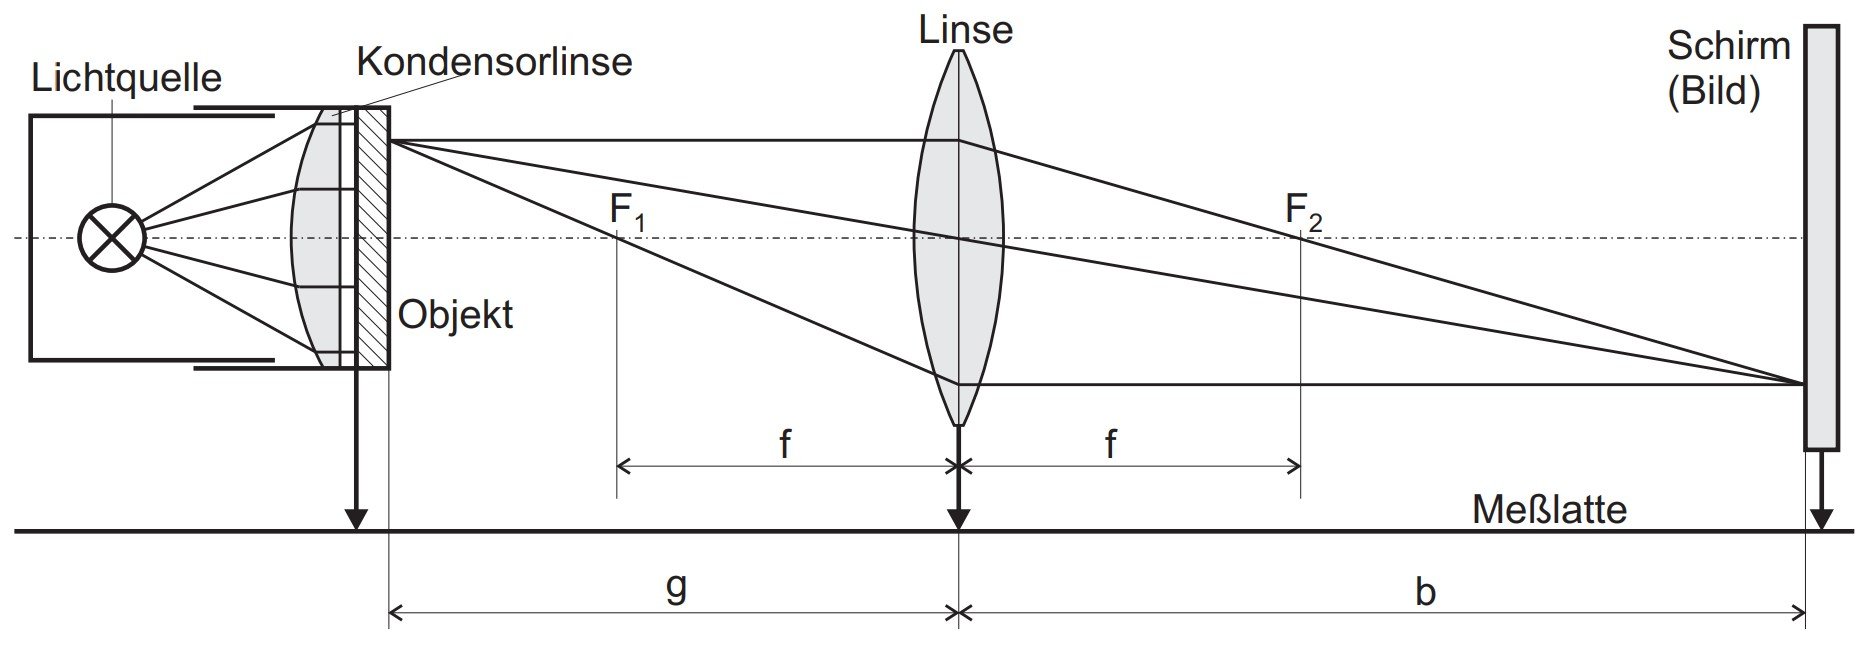
\includegraphics[width=0.6\linewidth]{nudes/laplace_theorie.jpg}
    \caption{Theoretischer Aufbau der Laplace'schen Methode. Bild aus Skriptum Dünne Linsen Seite 2 entnommen \cite{teachcenter2}. }
    \label{fig:laplace_theorie}
\end{figure}

\noindent
Mit der Formel \ref{eq:laplace} lässt sich aus der Bildweite $b$ und der Gegenstandweite $g$ die Brennweite $f$ berrechnen. 

\begin{equation}
    \label{eq:laplace}
    \centerline{$\frac{1}{f}=\frac{1}{g} + \frac{1}{b}$}
\end{equation}

\noindent
Ähnlich sieht es bei dem Bessel'schen Verfahren aus. Das Bild wird fokussiert. Durch bestimmung der Bildweite $b$ und der Gegenstandweite $g$ lässt sich der Gesamtabstand $a = g+b$ berrechnen. 
Die Linse wird verschoben, bis das Bild erneut scharf zu erkennen ist. Diese Strecke ist die Verschiebung $e$ wie in Abbildung \ref{fig:bessel_theorie} zu erkennen ist.  

\begin{figure}[H]
    \centering
    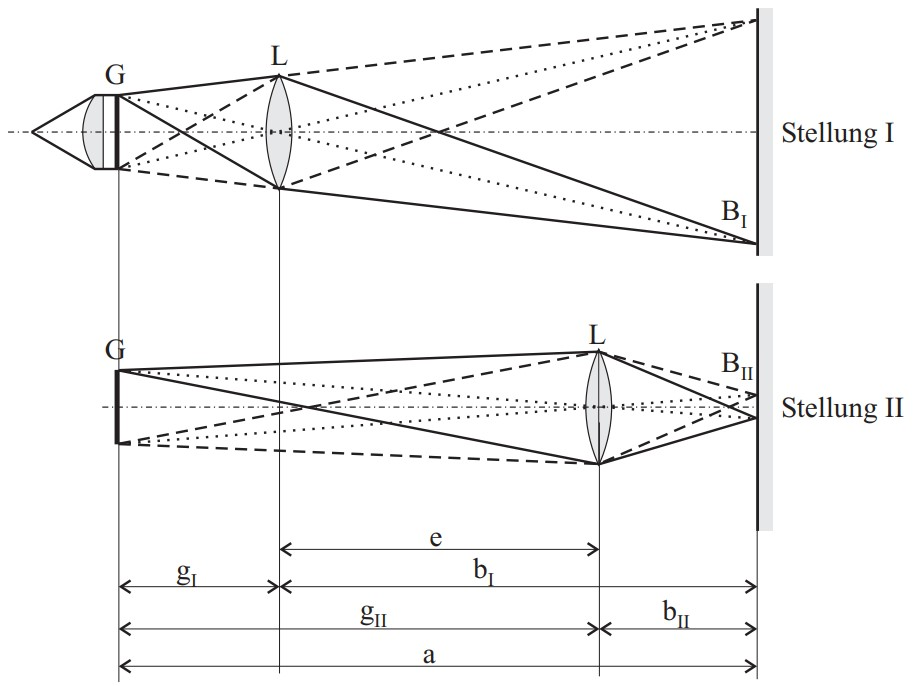
\includegraphics[width=0.6\linewidth]{nudes/bessel_theorie.jpg}
    \caption{Theoretischer Aufbau des Bessel'schen Verfahrens. Bild aus Skriptum Dünne Linsen Seite 3 entnommen \cite{teachcenter2}. }
    \label{fig:bessel_theorie}
\end{figure}

\noindent
Durch die Formel \ref{eq:bessel} lässt sich die Brennweite $f$ berrechnen. 

\begin{equation}
    \label{eq:bessel}
    \centerline{$\frac{1}{f}=\frac{1}{4} (\frac{a^2 - e^2}{a})$}
\end{equation}

\noindent
Um die Brennweite $f_s$ einer Zerstreuungslinse zu bestimmen benötigt man die Gegenstandweite $g'$ sowie die Bildweite $b$. 
Um diese zu bestimmen, wird die Linse in einer Gegenstandweite $g'$ zum Schirm aufgestellt. Durch Verschieben des Schirmes, bis das Bild scharf zu erkennen ist wird die Bildweite $b$ bestimmt. Die Brennweite $f_s$ wird mit folgender Formel bestimmt. 

\begin{equation}
    \label{eq:Zerstreuungslinse}
    \centerline{$\frac{1}{f_s}=\frac{1}{g'} + \frac{1}{b}$}
\end{equation}
\noindent
Hierbei ist jedoch anzumerken, dass die Brennweite $f_s$ ein negativer Wert ist. 
\\
\\
Da in diesem Versuch mehrere Messdaten aufgenommen werden, ist es wichtig, deren Mittelwert sowie die Standardabweichung zu berrechnen. 
In der Formel ist das $x$ Platzhalter für die Gegenstandweite $g$, $g'$, die Bildweite $b$ sowie die Verschiebung $e$. 
\\
Für die berechnung des Mittelwertes $\bar{x}$, benötigt man die Anzahl der Messversuche N sowie die einzelnen Weiten $x$. 

\begin{equation}
    \label{eq:Mittelwert}
    \centerline{$\bar{x} = \frac{1}{N} \sum_{i = 1}^{N} x_i $} 
\end{equation}

\noindent
Mit dem nun bekannten Mittelwert $\bar{x}$ lässt sich die Standardabweichung $\sigma_{x}$ berechnen. 

\begin{equation}
    \label{eq:Standardabweichung}
    \centerline{$\sigma_{x} = \sqrt{\frac{1}{N-1} \sum_{i = 1}^{N} (x_i - \bar{x})^2}$} 
\end{equation}
\section{Versuchsanordnung} %mit skizze kurz beschreiben ------------------------------
Die Versuche werden wie in den folgenden Bildern aufgebaut. Die Optischen Elemente befindet sich dabei auf einer Schiene, welche mit einem Lineal versehen ist. 


    \begin{figure}[H]
        \centering
        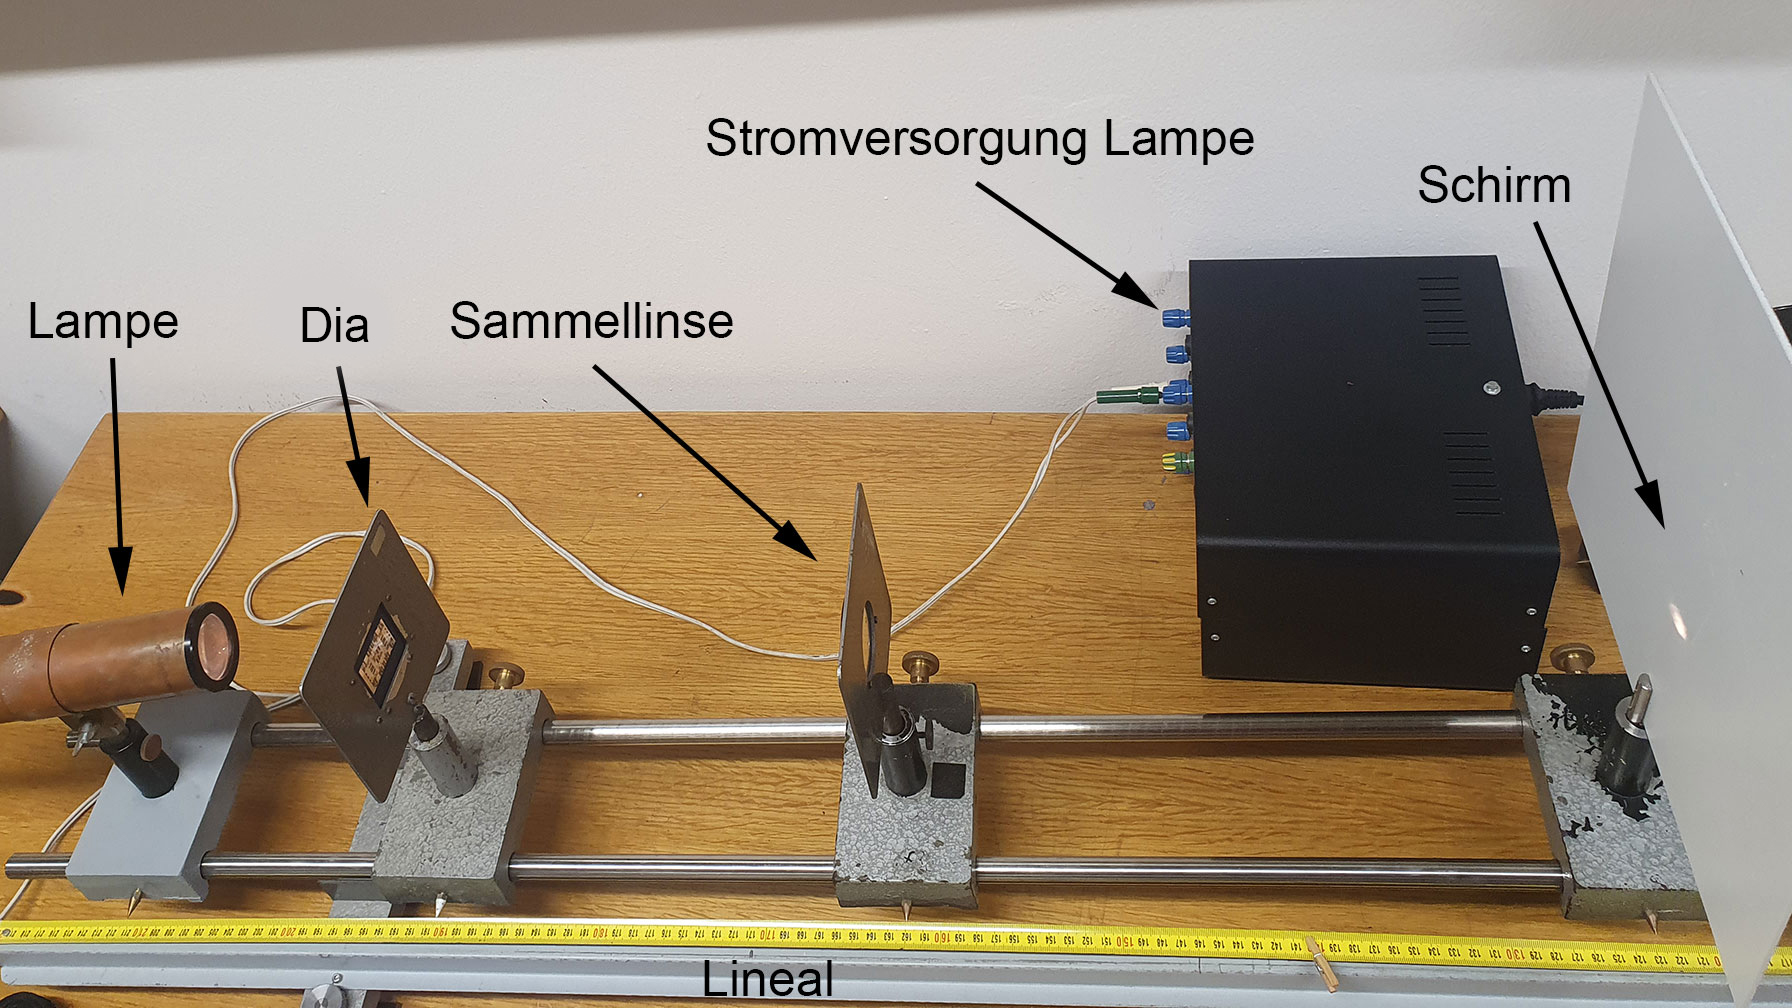
\includegraphics[width=0.6\linewidth]{nudes/komprimert/aufbau sammellinse.jpg}
        \caption{Aufbau der Versuche zur Bestimmung der Brennweite mit der Sammellinse. Beide Aufbauten sehen gleich aus. }
        \label{fig:aufbau Sammellinse}
    \end{figure}

    \begin{figure}[H]
        \centering
        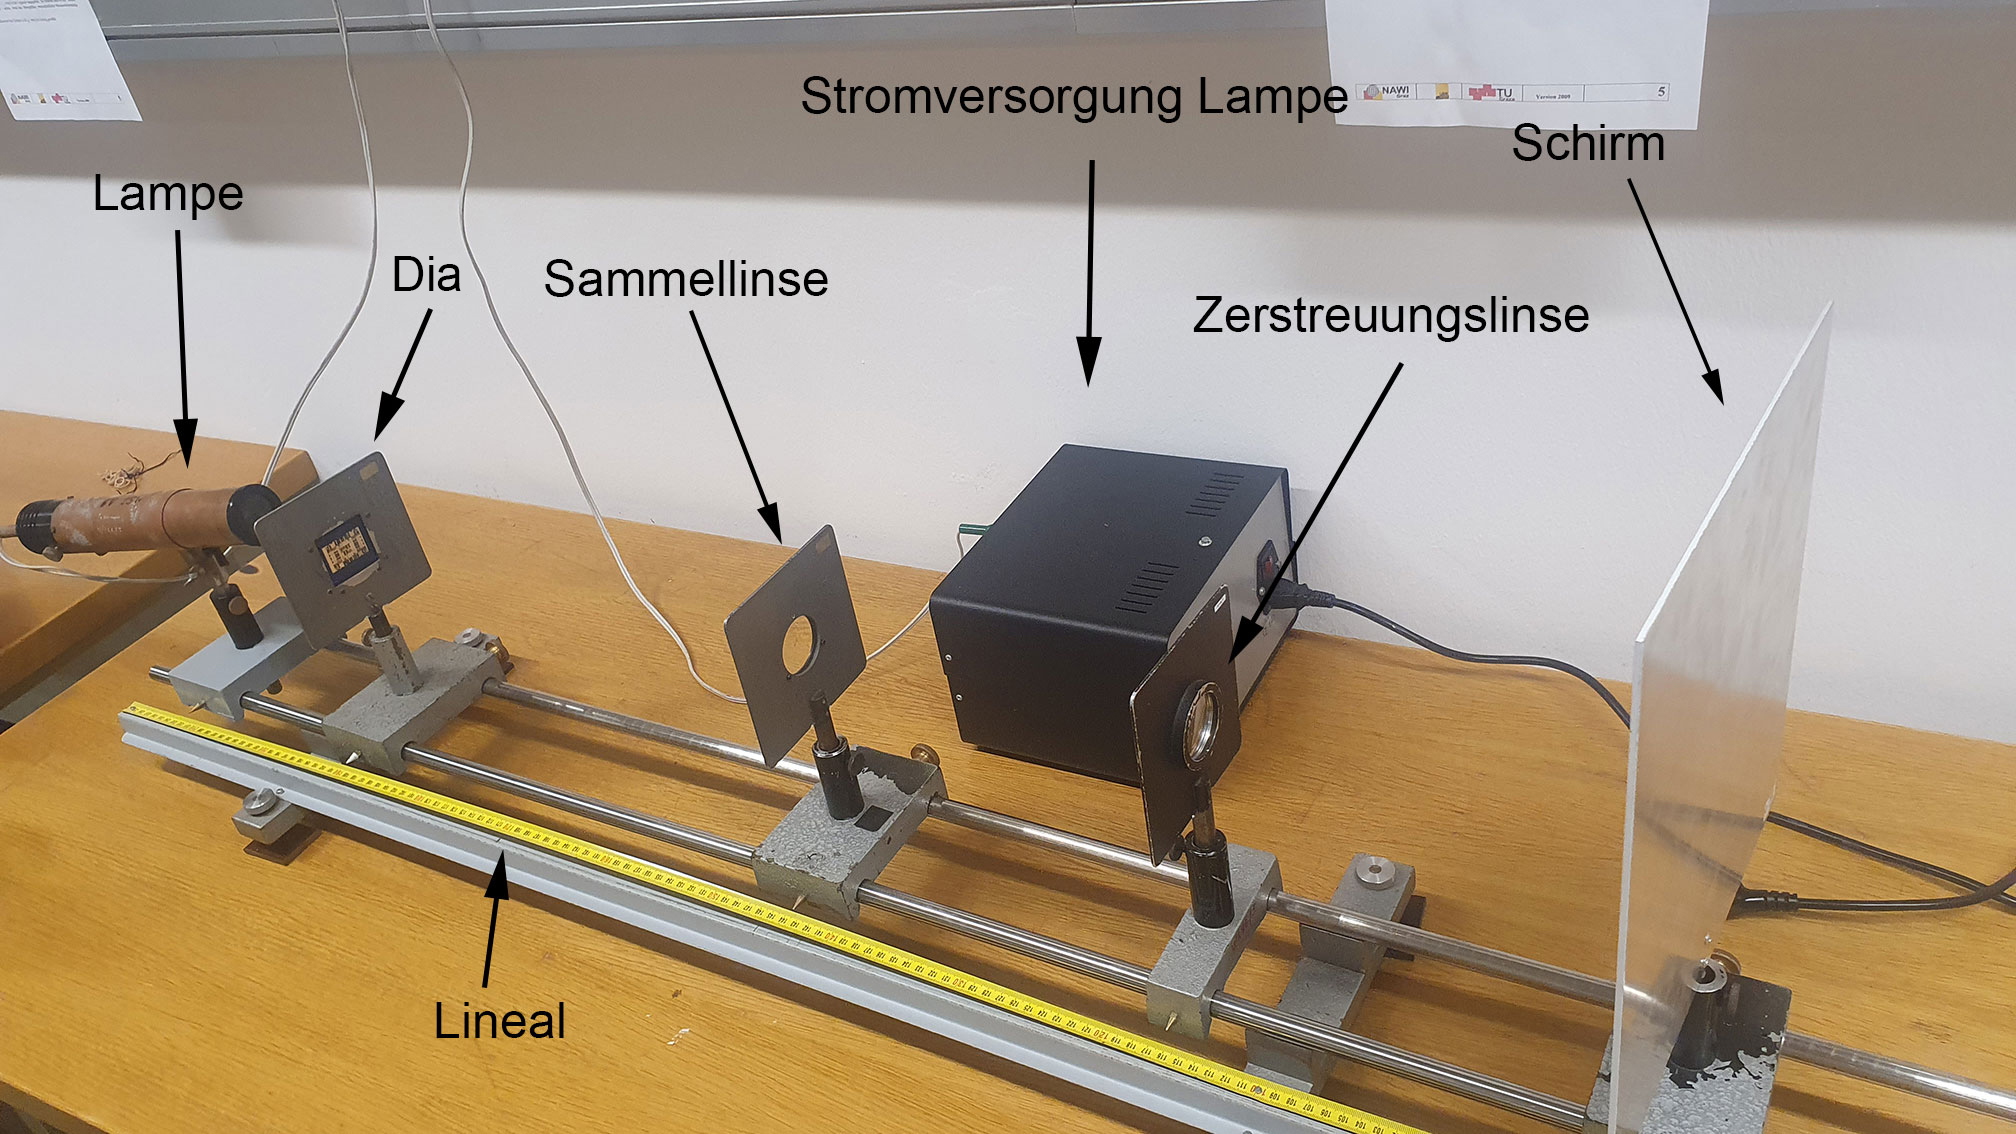
\includegraphics[width=0.6\linewidth]{nudes/komprimert/aufbau zerstreuungslinse.jpg}
        \caption{Versuchsaufbau für die Bestimmung der Brennweite der Zerstreuungslinse}
        \label{fig:aufbau Zerstreuungslinse}
    \end{figure}

    \begin{figure}[H]
        \centering
        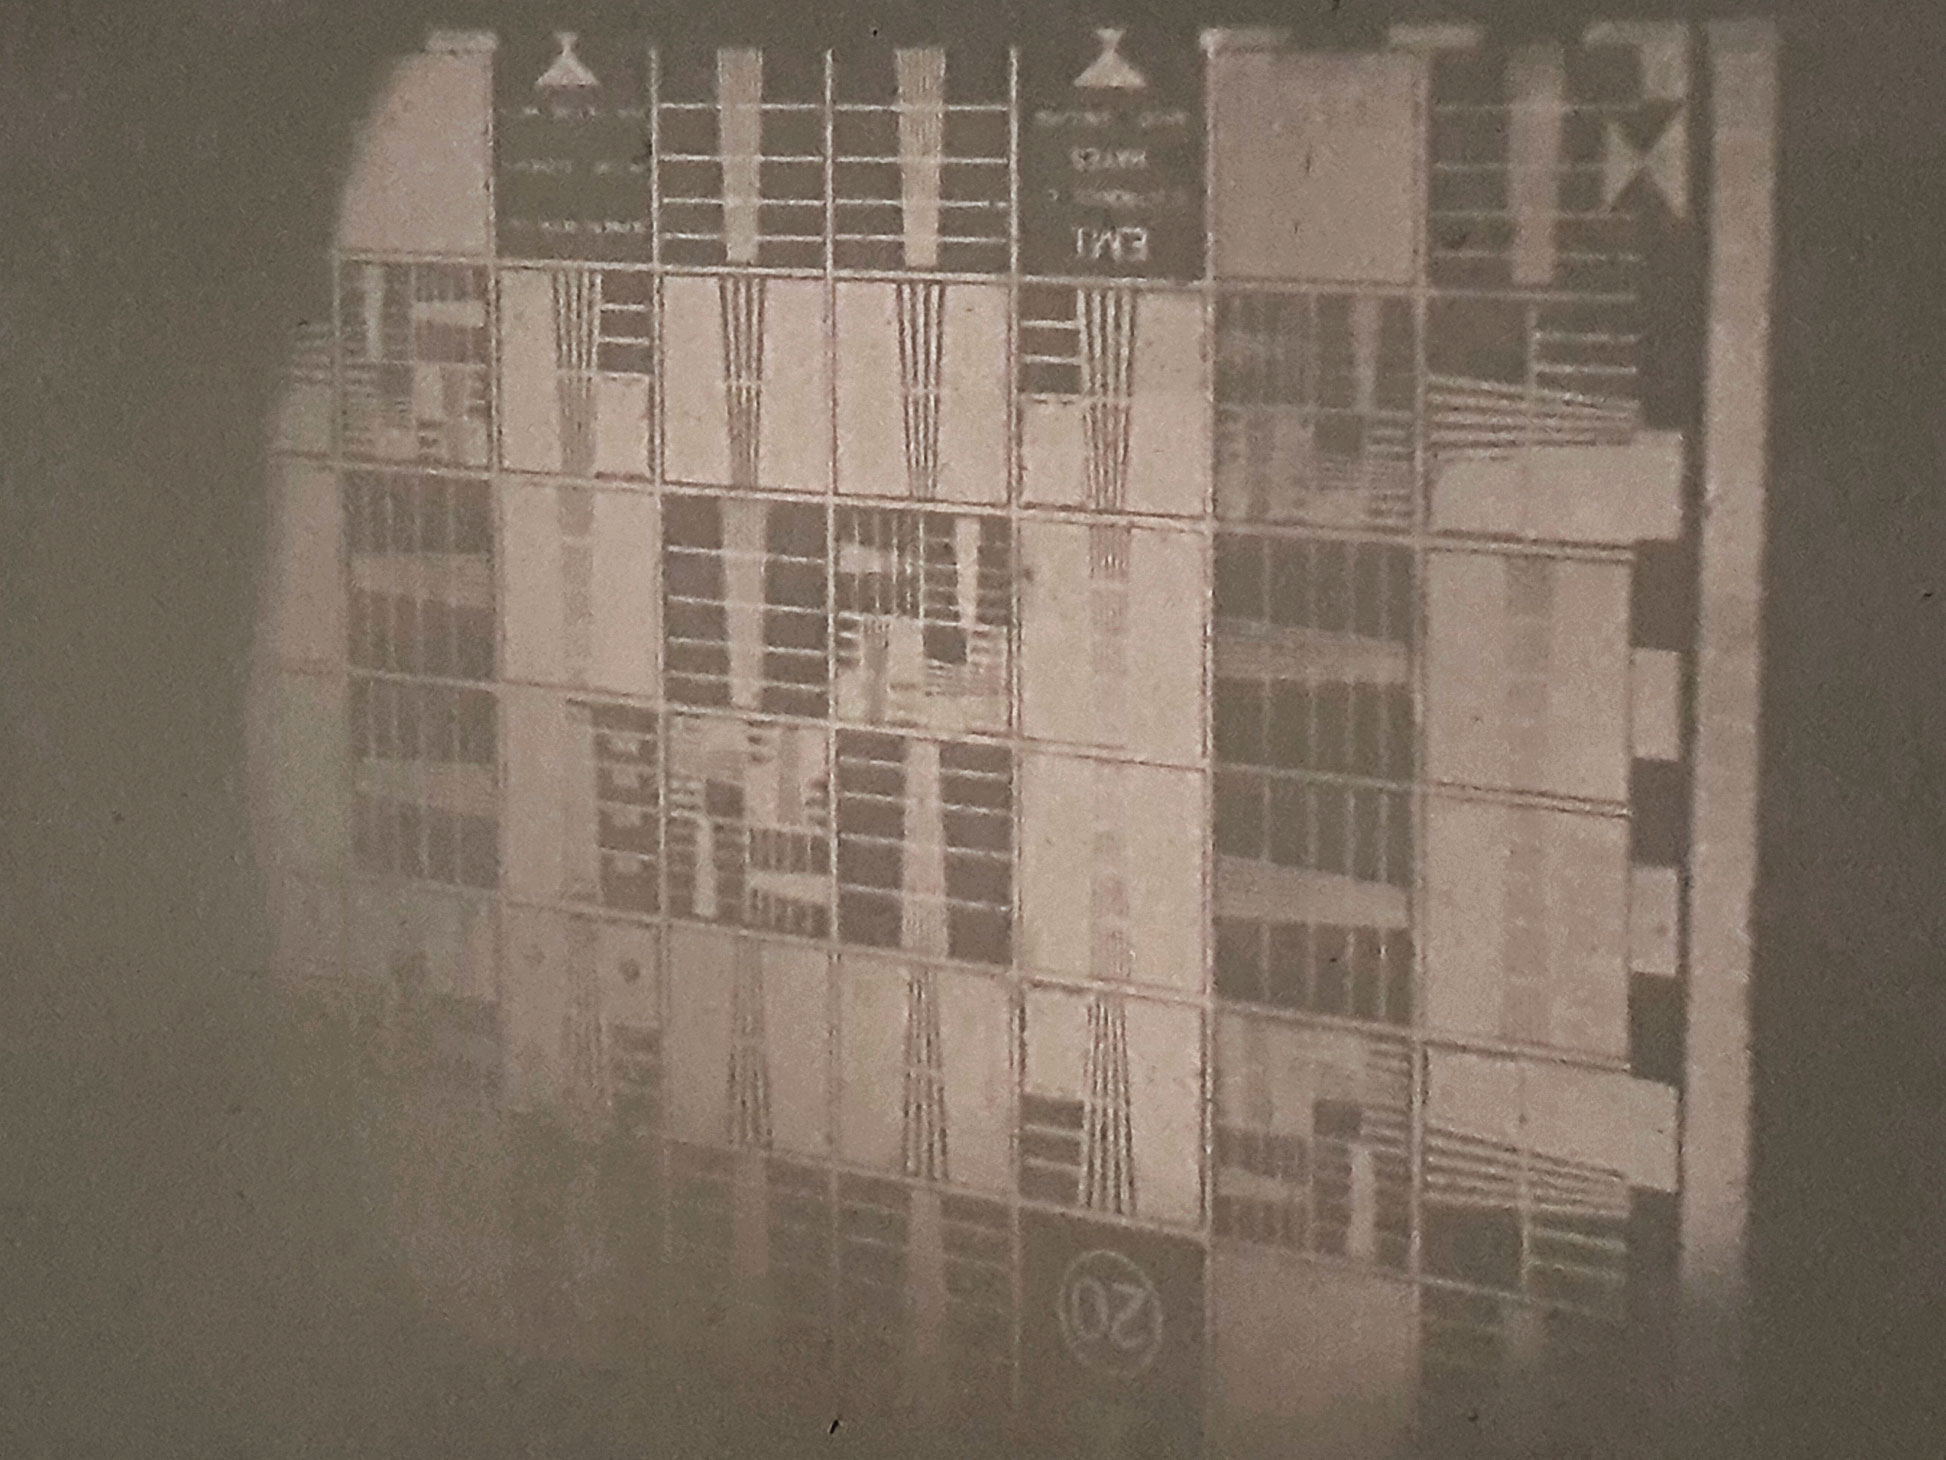
\includegraphics[width=0.6\linewidth]{nudes/komprimert/bild.jpg}
        \caption{Projeziertes, scharfgestelltes Bild}
        \label{fig:aufbau Bild}
    \end{figure}

\section{Geräteliste} %jo holt a listn ------------------------------

    \begin{table}[H]
        \centering
        \caption{Im Versuch verwendete Geräte und Utensilien.}
        \label{tab:geraete}
        \begin{tabular}{| l | l | l |}
            \hline
            Gerät  & Gerätenummer  & Unsicherheit \\
            \hline
            Lampe & {n.a} & {n.a} \\
            Sammellinse & {n.a} & {n.a} \\
            Zerstreuungslinse & {n.a} & {n.a} \\
            Schirm & {n.a} & {n.a} \\
            Lineal & {n.a} & $\pm 1.0 mm$ \\
        \end{tabular}
    \end{table}


\section{Versuchsdurchführung \& Messergebnisse} %nachvollziehbar und klar dargestellt ------------------------------
Um für den ersten Versuchsteil nach der Laplace'schen Methode die Gegenstandweite $g$ sowie die Bildweite $b$ zu bestimmen, werden insgesamt 10 Messversuche aufgestellt. 
Um diese zu bestimmen, wird mit dem auf der Schiene angebrachtem Lineal die Abstände von Linse zu Schirm ($b$) und Linse zu Lampe ($g$) gemessen. 
Der Schirm wird dabei jeweils um 10 cm verschoben. Die Linse wird so Verschoben, dass das Bild auf dem Schirm scharf abgebildet wird. Die Lampe hat dabei immer die gleiche Position. 

\begin{table}[H]
    \centering
    \caption{Messergebnisse der Abstände nach der Laplace'schen Methode für die Sammellinse. }
    \label{tab:messergebnisse Laplace}
    \begin{tabular}{| l | l | l | l |}
        \hline
        Nr.  & Schirm $\pm 0.1 $/ cm & Linse $\pm 0.1 $ / cm & Lampe $\pm 0.1 $ / cm \\
        \hline
        1  & 10.0   & 159.8  & 190.0 \\
        2  & 20.0   & 158.9  & 190.0 \\
        3  & 30.0   & 158.4  & 190.0 \\
        4  & 40.0   & 157.8  & 190.0 \\
        5  & 50.0   & 156.9  & 190.0 \\
        6  & 60.0   & 155.9  & 190.0 \\
        7  & 70.0   & 154.1  & 190.0 \\
        8  & 80.0   & 151.4  & 190.0 \\
        9  & 90.0   & 143.6  & 190.0 \\
        10 & 100.0  & 141.2  & 190.0 \\
        \hline
    \end{tabular}
\end{table}

\noindent
Im zweiten Teil wird nach dem Bessle'schen Verfahren die Brennweite bestimmt. 
Der Versuch wird insgesamt 5 mal wiederholt. Der Schirm wird immer um 10 cm verschoben, die Lampe hat immer die gleiche Positon. Aus deren differenz lässt sich auch der Gesamtabstand $a$ bestimmen. 
Die Linse wird so eingestellt, dass das Bild auf dem Schirm scharf abgebildet wird. Anschließend verschiebt man die Linse soweit zum Schirm, bis das Bild erneut scharf abgebildet wird. Diese Strecke ist die Verschiebung $e$. 

\begin{table}[H]
    \centering
    \caption{Messergebnisse der Abstände nach dem Bessel'schen Verfahren für die Sammellinse. }
    \label{tab:messergebnisse Bessel}
    \begin{tabular}{| l | l | l | l | l |}
        \hline
        Nr.  & Schirm $\pm 0.1 $ / cm &  Pos 1 $\pm 0.1 $ / cm & Pos 2 $\pm 0.1 $ / cm & Lampe $\pm 0.1 $ / cm \\
        \hline
        1  & 30.0   & 158.5 & 61.1  & 190.0 \\
        2  & 40.0   & 158.0 & 70.9  & 190.0 \\
        3  & 50.0   & 157.3 & 81.7  & 190.0 \\
        4  & 60.0   & 155.9 & 92.8  & 190.0 \\
        5  & 70.0   & 154.5 & 104.4 & 190.0 \\
        \hline
    \end{tabular}
\end{table}
Im dritten Teil, bei der Zerstreuungslinse, wird die Zerstreuungslinse auf einen Abstand gestellt. In einen beliebigen Abstand wird der Schirm aufgestellt. 
Die differenz dieser Abstände ist die Gegenstandweite $g'$. Nun wird der Schirm soweit entfernt, bis das Bild scharf zu erkennen ist. 
Die differenz zu der ersten Position des Schirmes ist die Bildweite $b$. 

\begin{table}[H]
    \centering
    \caption{Messergebnisse der Abstände für die Zerstreuungslinse. }
    \label{tab:messergebnisse Zerstreuungslinse}
    \begin{tabular}{| l | l | l | l |}
        \hline
        Nr.  & Linse $\pm 0.1 $/ cm & Schirm Pos. 1 $\pm 0.1 $ / cm & Schirm Pos. 2 $\pm 0.1 $ / cm \\
        \hline
        1  & 50.0   & 40.0 & 34.0 \\
        2  & 60.0   & 50.0 & 43.6 \\
        3  & 65.0   & 55.0 & 48.6 \\
        4  & 32.0   & 20.0 & 9.0  \\
        5  & 45.0   & 30.0 & 9.0  \\
        6  & 64.0   & 50.0 & 33.0 \\
        7  & 85.0   & 70.0 & 48.0 \\
        8  & 90.0   & 80.0 & 73.5 \\
        9  & 100.0  & 85.0 & 62.0 \\
        10 & 81.0   & 70.0 & 62.0 \\
        \hline
    \end{tabular}
\end{table}

\section{Auswertung und Unsicherheitsanalyse} %Nicht nur zahlen angeben ------------------------------

In der Auswertung werden zur erhöhten Genauigkeit durchgehend ungerundete Werte bis zu den Endergebnissen verwendet und nur zur Darstellung gerundet. \\
Zur Berechnung der Unsicherheiten wird, wenn nicht anders angegeben, die Größtunsicherheitsmethode verwendet.


\section{Diskussion} %diskussion der Unsicherheiten und Ergebnisse und evtl. verlgeich mit Literatur ------------------------------


\section{Zusammenfassung} %klare, übersichtliche vollständige beantwortung der Aufgabenstellung ------------------------------


\printbibliography[heading=bibintoc]
\end{document}
